% Options for packages loaded elsewhere
\PassOptionsToPackage{unicode}{hyperref}
\PassOptionsToPackage{hyphens}{url}
\PassOptionsToPackage{dvipsnames,svgnames,x11names}{xcolor}
%
\documentclass[
  10pt,
  letterpaper,
  twocolumn]{article}

\usepackage{amsmath,amssymb}
\usepackage{iftex}
\ifPDFTeX
  \usepackage[T1]{fontenc}
  \usepackage[utf8]{inputenc}
  \usepackage{textcomp} % provide euro and other symbols
\else % if luatex or xetex
  \usepackage{unicode-math}
  \defaultfontfeatures{Scale=MatchLowercase}
  \defaultfontfeatures[\rmfamily]{Ligatures=TeX,Scale=1}
\fi
\usepackage{lmodern}
\ifPDFTeX\else  
    % xetex/luatex font selection
  \setmainfont[]{Times New Roman}
\fi
% Use upquote if available, for straight quotes in verbatim environments
\IfFileExists{upquote.sty}{\usepackage{upquote}}{}
\IfFileExists{microtype.sty}{% use microtype if available
  \usepackage[]{microtype}
  \UseMicrotypeSet[protrusion]{basicmath} % disable protrusion for tt fonts
}{}
\makeatletter
\@ifundefined{KOMAClassName}{% if non-KOMA class
  \IfFileExists{parskip.sty}{%
    \usepackage{parskip}
  }{% else
    \setlength{\parindent}{0pt}
    \setlength{\parskip}{6pt plus 2pt minus 1pt}}
}{% if KOMA class
  \KOMAoptions{parskip=half}}
\makeatother
\usepackage{xcolor}
\setlength{\emergencystretch}{3em} % prevent overfull lines
\setcounter{secnumdepth}{-\maxdimen} % remove section numbering
% Make \paragraph and \subparagraph free-standing
\ifx\paragraph\undefined\else
  \let\oldparagraph\paragraph
  \renewcommand{\paragraph}[1]{\oldparagraph{#1}\mbox{}}
\fi
\ifx\subparagraph\undefined\else
  \let\oldsubparagraph\subparagraph
  \renewcommand{\subparagraph}[1]{\oldsubparagraph{#1}\mbox{}}
\fi


\providecommand{\tightlist}{%
  \setlength{\itemsep}{0pt}\setlength{\parskip}{0pt}}\usepackage{longtable,booktabs,array}
\usepackage{calc} % for calculating minipage widths
% Correct order of tables after \paragraph or \subparagraph
\usepackage{etoolbox}
\makeatletter
\patchcmd\longtable{\par}{\if@noskipsec\mbox{}\fi\par}{}{}
\makeatother
% Allow footnotes in longtable head/foot
\IfFileExists{footnotehyper.sty}{\usepackage{footnotehyper}}{\usepackage{footnote}}
\makesavenoteenv{longtable}
\usepackage{graphicx}
\makeatletter
\def\maxwidth{\ifdim\Gin@nat@width>\linewidth\linewidth\else\Gin@nat@width\fi}
\def\maxheight{\ifdim\Gin@nat@height>\textheight\textheight\else\Gin@nat@height\fi}
\makeatother
% Scale images if necessary, so that they will not overflow the page
% margins by default, and it is still possible to overwrite the defaults
% using explicit options in \includegraphics[width, height, ...]{}
\setkeys{Gin}{width=\maxwidth,height=\maxheight,keepaspectratio}
% Set default figure placement to htbp
\makeatletter
\def\fps@figure{htbp}
\makeatother

\usepackage{sdss2020}
\usepackage{url}
\usepackage{hyperref}
\usepackage{latexsym}
\usepackage{tabularx}
\usepackage{amsmath, amsthm, amsfonts}
\usepackage{algorithm, algorithmic}
\usepackage[table,dvipsnames]{xcolor} % ✅ Added "table" to support row coloring
\newcommand{\mt}[1]{{\textcolor{blue}{#1}}}
\newcommand{\svp}[1]{{\textcolor{RedOrange}{#1}}}
\makeatletter
\makeatother
\makeatletter
\makeatother
\makeatletter
\@ifpackageloaded{caption}{}{\usepackage{caption}}
\AtBeginDocument{%
\ifdefined\contentsname
  \renewcommand*\contentsname{Table of contents}
\else
  \newcommand\contentsname{Table of contents}
\fi
\ifdefined\listfigurename
  \renewcommand*\listfigurename{List of Figures}
\else
  \newcommand\listfigurename{List of Figures}
\fi
\ifdefined\listtablename
  \renewcommand*\listtablename{List of Tables}
\else
  \newcommand\listtablename{List of Tables}
\fi
\ifdefined\figurename
  \renewcommand*\figurename{Figure}
\else
  \newcommand\figurename{Figure}
\fi
\ifdefined\tablename
  \renewcommand*\tablename{Table}
\else
  \newcommand\tablename{Table}
\fi
}
\@ifpackageloaded{float}{}{\usepackage{float}}
\floatstyle{ruled}
\@ifundefined{c@chapter}{\newfloat{codelisting}{h}{lop}}{\newfloat{codelisting}{h}{lop}[chapter]}
\floatname{codelisting}{Listing}
\newcommand*\listoflistings{\listof{codelisting}{List of Listings}}
\makeatother
\makeatletter
\@ifpackageloaded{caption}{}{\usepackage{caption}}
\@ifpackageloaded{subcaption}{}{\usepackage{subcaption}}
\makeatother
\makeatletter
\@ifpackageloaded{tcolorbox}{}{\usepackage[skins,breakable]{tcolorbox}}
\makeatother
\makeatletter
\@ifundefined{shadecolor}{\definecolor{shadecolor}{rgb}{.97, .97, .97}}
\makeatother
\makeatletter
\makeatother
\makeatletter
\makeatother
\ifLuaTeX
  \usepackage{selnolig}  % disable illegal ligatures
\fi
\IfFileExists{bookmark.sty}{\usepackage{bookmark}}{\usepackage{hyperref}}
\IfFileExists{xurl.sty}{\usepackage{xurl}}{} % add URL line breaks if available
\urlstyle{same} % disable monospaced font for URLs
\hypersetup{
  pdftitle={Efficacy of Chemical Applications in Controlling Soil-Borne Pathogens of Soybean Using An In Vitro Approach},
  pdfauthor={Oluwafunmibi O. Fasanya},
  colorlinks=true,
  linkcolor={blue},
  filecolor={Maroon},
  citecolor={Blue},
  urlcolor={Blue},
  pdfcreator={LaTeX via pandoc}}

\title{Efficacy of Chemical Applications in Controlling Soil-Borne
Pathogens of Soybean Using An In Vitro Approach}
\author{
Oluwafunmibi O. Fasanya\\
Department of Statistics\\\\
{\tt \href{mailto:ofasanya2@unl.edu}{ofasanya2@unl.edu}}\\
}
\date{}



\begin{document}
\maketitle
\ifdefined\Shaded\renewenvironment{Shaded}{\begin{tcolorbox}[breakable, interior hidden, sharp corners, enhanced, borderline west={3pt}{0pt}{shadecolor}, boxrule=0pt, frame hidden]}{\end{tcolorbox}}\fi

\hypertarget{abstract}{%
\section{Abstract}\label{abstract}}

This study evaluates the impact of intercropping peppers with flowering
plants---Sunflower (\emph{Helianthus annuus}), Zinnia (\emph{Zinnia
elegans}), and Dianthus (\emph{Dianthus} spp.)---on pepper yield,
disease incidence, and insect population dynamics. Using a randomized
complete block design, yield measurements were recorded separately for
peppers located near flowering plants (``inner'') and those farther away
(``outer''). Results indicate significant yield differences across
treatments and highlight the agronomic potential of targeted
intercropping strategies.

\hypertarget{keywords}{%
\section{Keywords}\label{keywords}}

Peppers; Intercropping; Flowering plants; Yield; Disease incidence;
Insect populations

\hypertarget{project-reflection}{%
\section{Project Reflection}\label{project-reflection}}

On Thursday, February 13, from 11:45 AM to 1:00 PM, I had my initial
meeting with my client Kelvin Muchiri. He is currently a Master's
student working at the department of plant pathology and his advisor is
Garcia-Aroca Teddy. He is interested in investigating the efficacy of
chemical applications in controlling soil-borne pathogens of soybean.
The client indicated on the google form that they are interested in
performing a two-way ANOVA and Tukey-HSD tests for their data on
investigating the efficacy of chemical applications in controlling
soil-borne pathogens of soybean. To be able to follow the prepare
section of the POWER process, I mailed the client to ask for their
dataset and some information on their previously done analysis prior to
meeting since they indicated they have initially conducted some analysis
on the data. This helped with getting prepared for our meeting and also
helped implement the PREPARE stage of the power process. During the open
phase, we began by introducing ourselves and took some few minutes to
establish rapport between myself and the domain expert. Also, before I
asked them to give me a more detailed explanation of their project
again, we briefly discussed their deadlines, their expectations and I
also took the time to explain how I'm going to be helping on the
project, after which we transitioned into the work phase. I believe this
phase was quite helpful as it kind of set a collaborative and welcoming
tone which made the domain expert feel more comfortable. During the main
part of the consultation, which is the work phase, I asked the domain
expert to give me detailed explanation of how they conducted the
experiment again as it would help me in determining the right approach
to model their data. The domain expert ability to clearly provide a
pictorial representation of their design was very helpful as it made me
see exactly what was going on in their experiment. While describing his
experiment, I noticed he had some nested structure he was not aware of
and also his dataset contains a lot of zero's which he also was not
bothered about. So I had to explain what a crossed and nested structure
is and also asked more question about the information the zero-values
were providing. The domain expert showed flexibility and willingness to
collaborate, as they were open to suggestions with regards to analyzing
their dataset in alignment with the way their experiment was designed.
Their consistent engagement, insightful questions and calling my
attention to explain what they do not understand reflected their trust
in our expertise and a readiness to co-work with me on the analysis.
After the initial meeting a document summarizing the experiment
objectives and design was sent to the domain experts in order to be sure
everyone is aware of the work we've gotten so far and so to ask some
other questions that came up when I was reflecting on our meeting.\\
In general, I had an amazing experience working on this project with the
domain-expert. Having the opportunity to collaborate directly with
domain experts was a really great experience. I learned so much just
listening to them explain their research approach and methodology. It
was fascinating to see how they conducted their work in practice. Being
part of a real-world project rather than just theoretical exercises
really deepened my understanding and made the whole experience
worthwhile.

\hypertarget{introduction}{%
\section{Introduction}\label{introduction}}

Soybeans is a food and oilseed crop which is rich in both protein and
edible oil. It is a major source of protein for both human and livestock
but is prone to many disease that could cause a significant decrease in
yield. As reported by (S Navi \& Rajasab, 2016) in their paper, in 2013,
soybean was grown in 70 countries with an annual production of 268
million metric tons with United states (31\%), Brazil (31\%) and
Argentina (19\%) being the highest producer of soybeans. However, report
from the USDA website showed that in 2024/2025 (Marketing Year 2024 from
September -- August), Brazil is currently the largest producer of
soybeans with about 169 million metric tons, followed by USA with about
118.84 million metric tons and the third largest producer is Argentina
with 49 Million metric tons. The production from these three countries
makes up 80\% of the global population of soybeans around the world with
40\% from Brazil, 28\% from USA, and 12\% from Argentina (USDA, 2025).
This reduction in yield of soybeans varies over the years as there are
many factors that could affect grain yields and some of them include
environment, production practices, and a variety's susceptibility to
disease (Allen et al., 2023). In 2022, About 3 out of 4 the soybeans
production in the United States comes from the northern states
(Illinois, Indiana, Iowa, Kansas, Michigan, Minnesota, Nebraska, New
York, North Dakota, Ohio, Pennsylvania, South Dakota, and Wisconsin) and
all of these states jointly has a yield loss of 71.3\% of the total
soybeans loss in 2022. Seedling diseases due to Fusarium, Pythium,
Phomopsis and Rhizoctonia are one of the major causes of soybeans loss
in 2022 (Allen et al., 2023). Despite the advancements in soybean
cultivation practices, plant pathogens continues to limit soybean
yields. According to farm journal, the following soil-borne fungal
pathogens (Fusarium, Rhizoctonia, Pythium, and Phytophthora) are some of
the major causes of seedlings blights in soybeans and they are
attributed to the loss of about 6 million bushels of soybeans in the
United State and Canada in 2023 (farmjournal, 2025).\\
In Nebraska, the largest producer of beef and pork, Soybeans is one of
the major ingredient used in the beef and pork production. However,
Nebraska experiences an estimated annual loss exceeding 9 million
bushels due to pathogenic organisms (CropWatch, n.d.). According to (S
Navi \& Rajasab, 2016), several fungal pathogens such as Colletotrichum
truncatum, Fusarium virguliforme, Macrophomina phaseolina, Pythium
irregulare, Rhizoctonia solani, and Sclerotinia sclerotiorum, are major
contributors to soybean seedling diseases, which leads to decrease in
soybeans yield. Their study evaluated the efficacy the following
fungicides: Foliar fungicides picoxystrobin (Aproach®), fluoxastrobin
(Evito), pyraclostrobin (Headline EC) and azoxystrobin (Quadris),
pyraclostrobin + fluxapyroxad (Priaxor), trifloxystrobin +
prothioconazole (Stratego YLD), and fluxapyroxad (Sercadis) on the
following pathogens: Colletotrichum truncatum (CT), Fusarium
virguliforme (FV), Macrophomina phaseolina (MP), Pythium irregulare
(PI), Rhizoctonia solani (RS), Sclerotinia sclerotiorum (SS), Septoria
glycines (SG) using an in vitro culture plug method. The result showed
that, all of the fungicide except Sercadis reduced the growth of CT
isolates. Headline EC, Priaxor, and Stratego YLD significantly reduced
the growth of Fusarium virguliforme (FV), Macrophomina phaseolina (MP),
Rhizoctonia solani (RS), and Sclerotinia sclerotiorum (SS). Sercadis was
very effective against Rhizoctonia solani (RS) while Aproach and Quadris
were effective against Fusarium virguliforme (FV). The objective of this
study is to investigate the efficacy of chemical applications in
controlling soil-borne pathogens of soybean and to look at the tolerance
of the various pathogens to fungicide at different dose level.

\hypertarget{materials-and-method}{%
\section{Materials and Method}\label{materials-and-method}}

This experiment was conducted toThe fungicide used was incorporated into
the growth medium (petri dish) to ensure there was homogeneous
distribution of this chemical across the different fungal species. To
achieve this, they collected data based on the species of pathogens
(isolates), different types of fungicide treatments and also at varying
dose level. This experiment was setup this way so that it would mimic
how the different fungicide would react with the pathogens in the
natural soil conditions. The details of the experimental design is given
below: Soybeans Pathogens The following isolates (species) were used in
this study: Diaporthe longicolla, Fusarium oxysporum, Fusarium solani
and Rhizoctonia solani. Fungicide The following fungicide was used:
DelaroComplete 3 active ingr (Proth+Trif+Fluop), Endura 1 active
ingredients (Boscalid), Quadris 1 active ingredients (Azoxystrobin),
Topguard 1 active ingredient (Flutriafol), and Topguard EQ 2 active
ingredient (Flut+Azoxys) Each of the fungicide treatments got 3 levels
of doses (Dose in mg/ml) with one control.

\begin{table}[h!]
\scriptsize
\centering
\caption{Fungicide active ingredients and their dose levels (mg/ml).}
\begin{tabular}{|l|c|c|c|c|}
\hline
\textbf{Fungicide} & \textbf{Dose 1} & \textbf{Dose 2} & \textbf{Dose 3} & \textbf{Control} \\
\hline
Proth+Trif+Fluop & 6.292 & 0.6292 & 0.06292 & 0 \\
Boscalid & 4.011 & 0.4011 & 0.04011 & 0 \\
Azoxystrobin & 6.1036 & 0.61036 & 0.061036 & 0 \\
Flutriafol & 5.7975 & 0.57975 & 0.057975 & 0 \\
Flut+Azoxys & 4.9128 & 0.49128 & 0.049128 & 0 \\
\hline
\end{tabular}
\end{table}

\textbf{Response:} Radial growth rate of pathogens were measured in the
presence and absence (dose = 0) of fungicides.\\
Each petri dish had 4 measurements (radial growth), which indicates that
fungi often grow unevenly, so taking multiple measurements improves
precision.

\begin{table}[h!]
\scriptsize
\centering
\caption{Skeleton ANOVA (split-Plot Factor Factor Nested in Whole-plot factor)}
\begin{tabular}{|l|c|}
\hline
\textbf{SV} & \textbf{df} \\
\hline
Treatment & (5-1) = 4 \\
\hline
Dose(Treatment) & (4-1)*5 = 15 \\
\hline
Species & (4-1) = 3 \\
\hline
Treatment*Species & (5-1)*(4-1) = 12 \\
\hline
Species*Dose(Treatment) & 3*15 = 45 \\
\hline
Error(Dish(Dose*Species*Treatment)) & (3-1)*(4*4*5) = 160 \\
\hline
\end{tabular}
\end{table}

\vspace{-0.3cm}
The model specification is given as:
\begin{multline}
\text{Avg\_Measurement} = \text{Species} \times \text{Treatments} + \\
(1|\text{Dose:Treatments}) + (1|\text{Species:Dose:Treatments})
\end{multline}

\vspace{-0.3cm}
Where:
\begin{itemize}
\setlength{\itemsep}{0pt}
\setlength{\parskip}{0pt}
\item \text{Species} \times \text{Treatments} is the fixed effects interaction which enables us to determine how different fungal species respond to different fungicide treatments.
\item (1|\text{Dose:Treatments}): This nested structure accounts for random variability due to different doses within each treatment.
\item (1|\text{Species:Dose:Treatments}): This nested structure accounts for the random variation in species responses within specific dose-treatment combinations.
\end{itemize}

\vspace{-0.1cm}
\subsection*{Two-Part Model (Zero-Inflated Gamma)}
\vspace{-0.2cm}

We model the growth of the fungus (mix of zero and positive values (semicontinuous)) using the two-part model as shown below
\begin{equation}
f(y) = (1 - \pi) I(y = 0) + \pi G_\theta(y| y > 0)
\end{equation}

\vspace{-0.3cm}
where $\pi = logit(x\beta) = log (\frac{x\beta}{1-x\beta})$, this is the parameters used in modeling the Probability of fungal growth greater than zero. $G_\theta(y| y > 0)$ follows a Gamma $(\alpha,\beta)$ distribution with $\alpha$ as the shape parameter, and $\beta$ as the scale parameter. The zero-inflated gamma distribution is given as ZIGamma$(\pi, \alpha,\beta)$, where $\pi$ is the probability that the fungus die (y = 0), while $\alpha$ and $\beta$ provides information about the gamma distribution, the non-zero part of the model. For the zero-inflated gamma model, the probability that the fungus does not die is modeled using the logistic regression while the distribution of the non-zero i.e. growth of fungus is modelled using the gamma distribution with a log-link.

\section*{Model Structure}
\vspace{-0.2cm}
This study performed a zero-inflated Gamma model to look at the effects of species, and treatments on the average fungal growth (positive continuous measurements with an excess of zeros), while also accounting for the nested structure of dose. This model was fitted using the ``glmmTMB'' package in R.
\vspace{-0.2cm}
\begin{itemize}
\setlength{\itemsep}{0pt}
\setlength{\parskip}{0pt}
\item The nonzero part (positive fungal growth) was modelled using a Gamma distribution 
\item The zero-inflated part which model the probability of an observation being structurally zero was modelled using a logistic regression
\end{itemize}
\vspace{-0.3cm}
The gamma component consists of:
\vspace{-0.3cm}
\begin{itemize}
\setlength{\itemsep}{0pt}
\setlength{\parskip}{0pt}
\item main effect of species, and treatment, 
\item interaction between species and treatment, and 
\item the random effects for dose nested within treatment.
\end{itemize}
\vspace{-0.3cm}
The zero-inflated component includes only the intercept assuming a constant probability of excess zeros across groups.
\vspace{-0.3cm}
\begin{equation}
\vspace{-0.3cm}
Y_{ijkl} \sim Zero\ inflated\ Gamma\ (\pi_{ijkl}, \alpha, \beta), \text{where}
\end{equation}
\vspace{-0.3cm}
\begin{itemize}
\setlength{\itemsep}{0pt}
\setlength{\parskip}{0pt}
\vspace{-0.3cm}
\item $Log(E[Y_{ijkl}|Y_{ijkl} > 0]) = \mu + Species_i + Treatment_j + (Species \times Treatment)_{ij} + (1|Dose:Treatment) + (1|Species:Dose:Treatment)$
\item $Logit(\pi_{ijkl}) = \beta_0$
\item $\epsilon_{ijkl} \sim Gamma(\alpha, \beta)$
\end{itemize}
\vspace{-0.3cm}
$Y_{ijkl}$ is the average measurement for the $i$th species, $j$th fungicide treatment, $k$th dose and $l$th dish.
$\mu$ is the baseline log mean fungal growth
$\epsilon_{ijkl}$ is the overall error term.
\subsection*{Zero Inflation Model}
$\beta_0$ is the intercept

\hypertarget{explanatory-analysis}{%
\subsection{Explanatory Analysis}\label{explanatory-analysis}}

Figure 1 shows the distribution of fungal growth across different type
of treatments. Since the fungus spreads out like a circle as they grow,
four measurements were taken: from the center to the top (measurement
1), center to the right (measurement 2), center to bottom (measurement
3), and center to the left (measurement 4). Figure 1 thus shows that the
mean growth across the various measurements were similar across
directions, thus we took the average of the four values for each
experimental unit. Figure 2 shows the average fungal growth across
different treatments. The plot shows Quadris 1 active ingredient has the
highest average fungal growth followed by Endura 1 active ingredient,
Topguard EQ 2 active ingredient and Topguard 1 active ingredient. As
also observed from figure 3, Quadris 1 active ingredient (Azoxystrobin)
showed the highest median fungal growth and the greatest variability,
this suggests that this treatment was less effective in fungal control
compared to the other treatments. Endura 1 active ingredient (Boscalid)
had the next highest median growth but exhibited slightly less
variability. Topguard 1 active ingredient (Flutriafol), Topguard EQ 2
active ingredients (Flutriafol + Azoxystrobin), and DelaroComplete 3
active ingredients (Prothioconazole + Trifloxystrobin + Fluopyram) had
lower median fungal growth, which suggest better overall control of
fungal spread.

\begin{figure}

{\centering 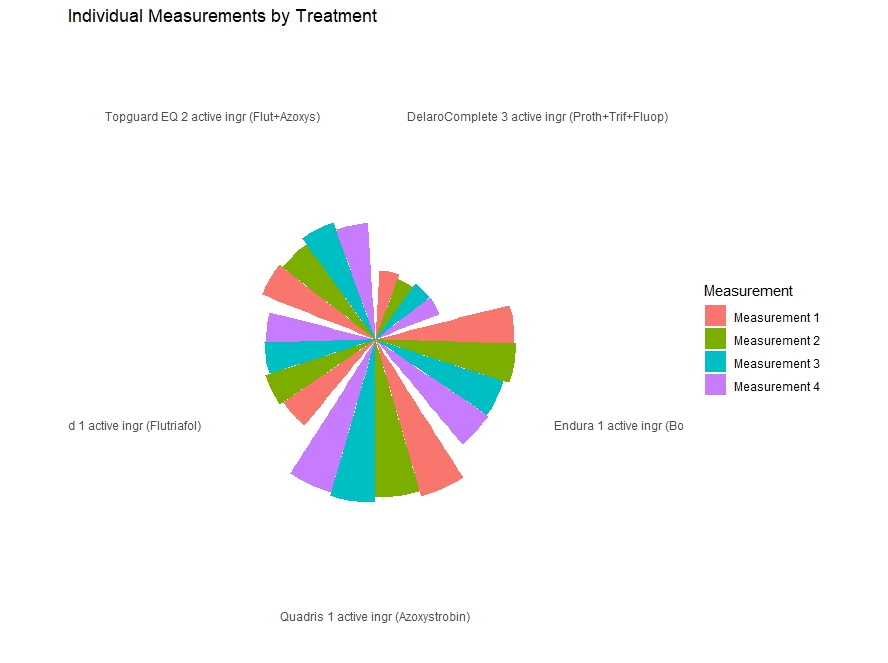
\includegraphics[width=0.5\textwidth,height=\textheight]{Fig1.jpeg}

}

\caption{Radial growth by Treatment}

\end{figure}

\begin{figure}

{\centering 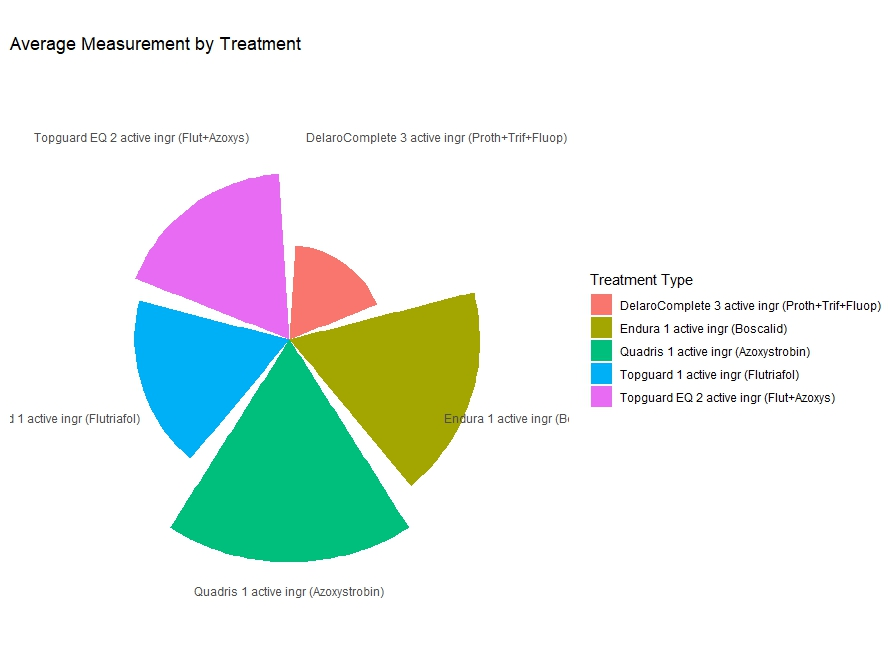
\includegraphics[width=0.5\textwidth,height=\textheight]{Fig3.jpeg}

}

\caption{Average Radial growth by Treatment}

\end{figure}

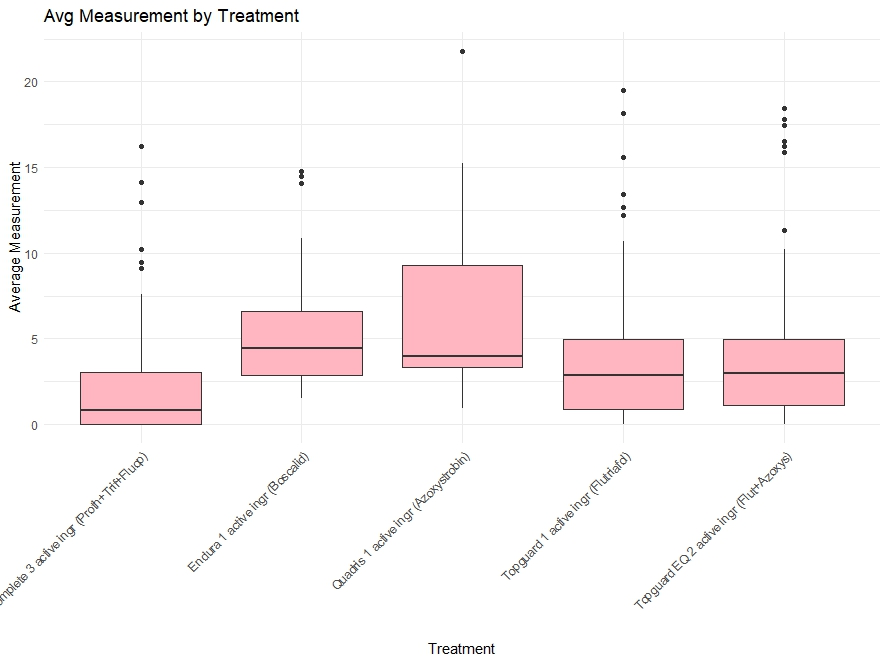
\includegraphics[width=0.5\textwidth,height=\textheight]{Fig5.jpeg}
Figure 4 shows the distribution of fungal growth across different
species. As also observed in Figure 1, the the mean growth across the
various measurements were similar across directions, Figure 5 shows the
average fungal growth across species. Fusarium oxysporum grows the
highest, followed by Rhizoctonia solani, Fusarium solani and Diaporthe
longicolla. Also, from figure 6, we were able to confirm that. Fusarium
oxysporum has the highest growth under the experimental conditions,
while Diaporthe longicolla has the least.

\begin{figure}

{\centering 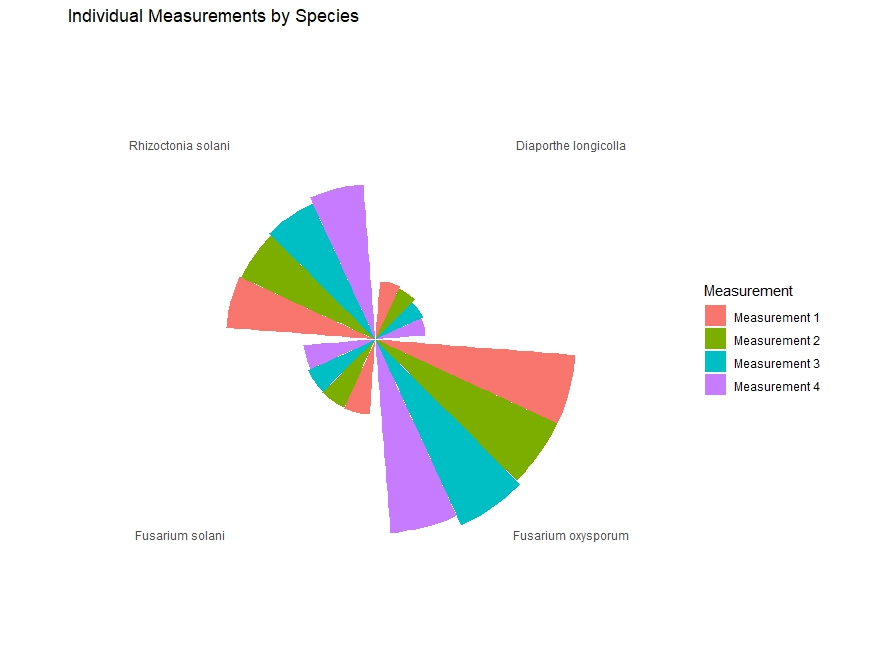
\includegraphics[width=0.5\textwidth,height=\textheight]{Fig2.jpeg}

}

\caption{Radial growth by Species}

\end{figure}

\begin{figure}

{\centering 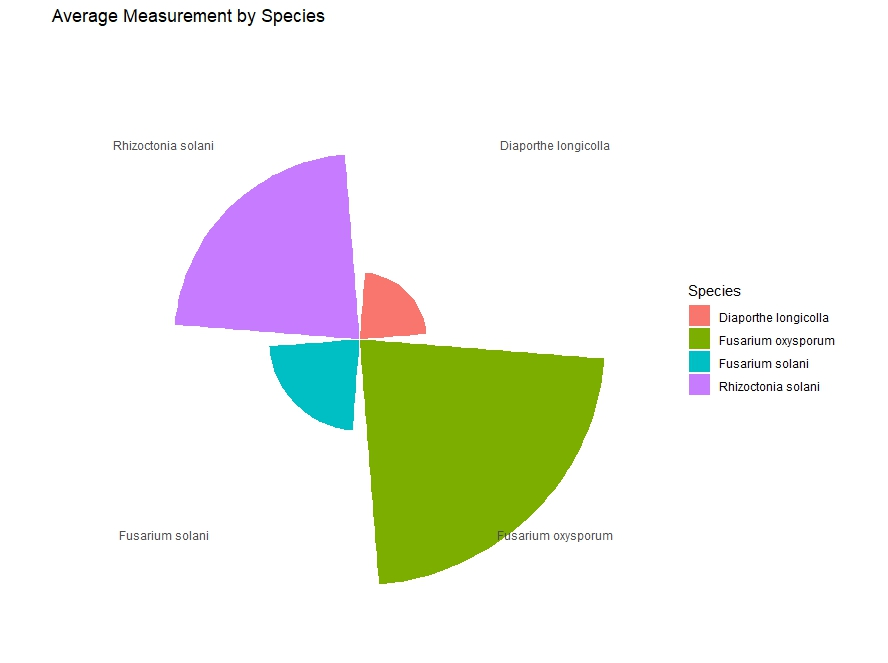
\includegraphics[width=0.5\textwidth,height=\textheight]{Fig4.jpeg}

}

\caption{Radial growth by Species}

\end{figure}

\begin{figure}

{\centering 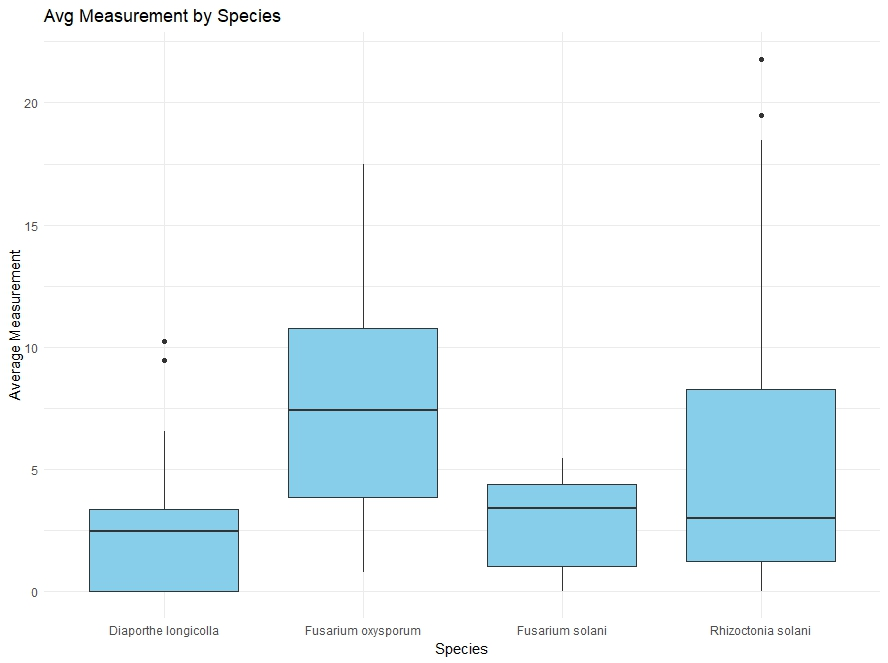
\includegraphics[width=0.5\textwidth,height=\textheight]{Fig6.jpeg}

}

\caption{Radial growth by Species}

\end{figure}

Figure 7 shows the distribution of average fungal growth measurements
across different fungicide dose levels, split by fungal species. For
Diaporthe longicolla species, the following dose: 6.292, 5.7975, 4.9128,
0.6292, 0.57975, 0.49128, 0.06292, and 0.057975, resulted in complete
death of fungal growth, as shown by an absence of measured growth
i.e.~growth = 0. Also, for Fusarium solani, the following doses: 6.292,
0.6292, and 0.06292 completely killed the development of the fungus.
However, for Fusarium oxysporum, we saw some resistance to the fungicide
treatment dose as there were observable groth of the fungus across all
dose level. Same was also observed for Rhizotonia solani.

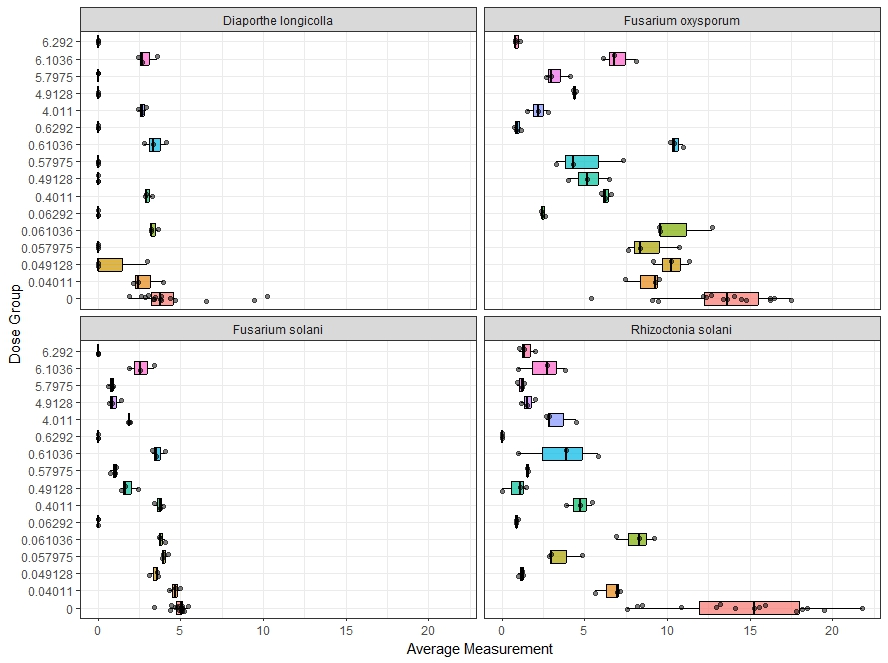
\includegraphics[width=0.5\textwidth,height=\textheight]{Fig7.jpeg}
Figure 8 shows the distribution of average fungal growth across
different fungicide dose levels, split by fungicide treatment. This plot
showed that specific dose was used in each of the treatment, this showed
the nested structure of dose within treatment. From the plot, we
observed that across all the treatments, fungal growth decreased with
increase in the level of the fungicide dose.

\begin{figure}

{\centering 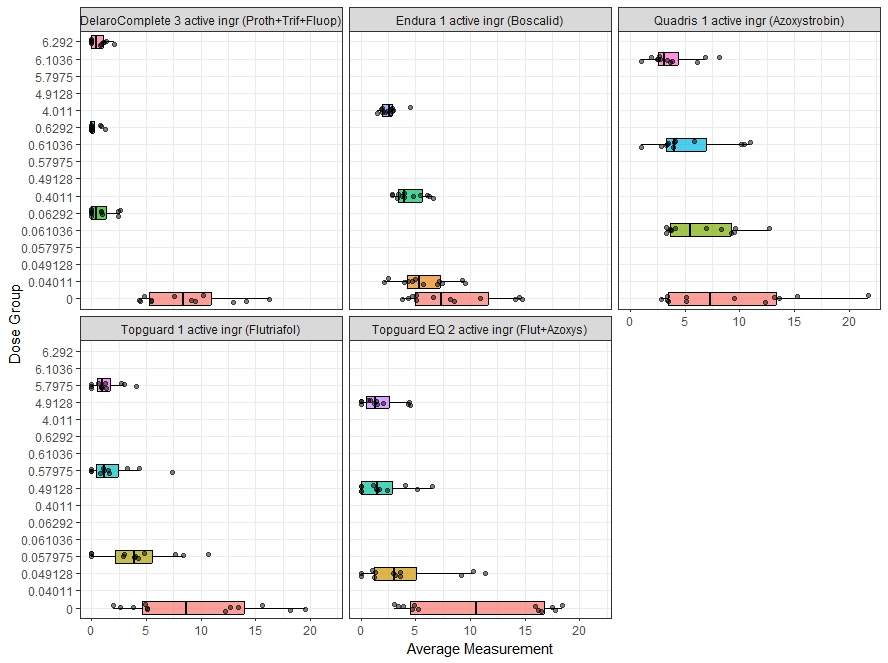
\includegraphics[width=0.5\textwidth,height=\textheight]{Fig8.jpeg}

}

\caption{Radial growth by Species}

\end{figure}

Figure 9 shows the histogram of the average fungal measurements. The
distribution is right-skewed, with a high concentration of observations
clustered at lower growth values.

\begin{figure}

{\centering 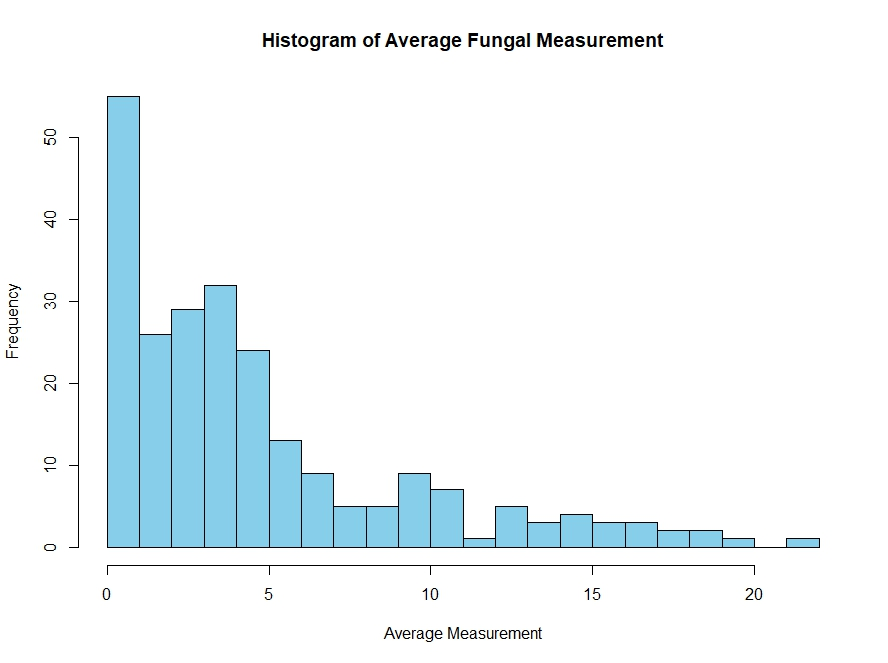
\includegraphics[width=0.5\textwidth,height=\textheight]{Fig9.jpeg}

}

\caption{Radial growth by Species}

\end{figure}

\hypertarget{advanced-analysis}{%
\section{Advanced Analysis}\label{advanced-analysis}}

The major goal of performing this experiment is to determine the
effectiveness of fungicides against resistant pathogens.

\hypertarget{random-effect-structure}{%
\section{Random Effect Structure:}\label{random-effect-structure}}

This part of the result shows the nested structure variability in both
the conditional and the zero-inflated model.

\hypertarget{conditional-model-variance-components}{%
\section{Conditional Model Variance
Components:}\label{conditional-model-variance-components}}

\begin{figure}

{\centering 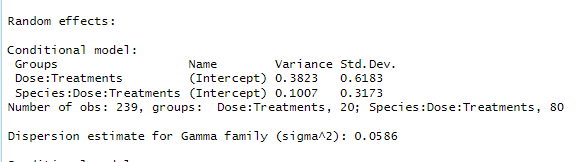
\includegraphics[width=0.5\textwidth,height=\textheight]{Fig10.png}

}

\caption{Radial growth by Species}

\end{figure}

Dose:Treatments: Variance = 0.3823 (SD = 0.6183)
Species:Dose:Treatments: Variance = 0.1007 (SD = 0.3173)

This result shows the variability in the pathogens growth for dose
nested in treatment and also for species crossed with treatment nested
within dose i.e.~variability in how each species respond to the
different fungicide (dose treatment combination). The variation in the
growth of the pathogens due to the random effect of dose nested within
treatments is 0.3823 and the variation in the growth of the pathogens
due to the random effect of species crossed with treatments nested
within dose is 0.1007.

\begin{figure}

{\centering 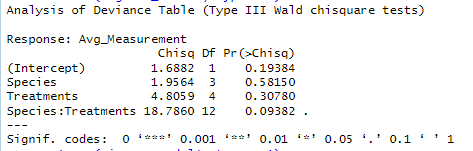
\includegraphics[width=0.5\textwidth,height=\textheight]{Fig11.png}

}

\caption{Radial growth by Species}

\end{figure}

\hypertarget{fixed-effect-structure}{%
\section{Fixed Effect Structure:}\label{fixed-effect-structure}}

The result above shows the ANOVA table for the effect of species,
treatments and the interaction between treatments and species for the
gamma regression section of the zero-inflated model. The result showed
that a marginal significant interaction between species and treatment (p
\textgreater{} 0.05). We looked further to see which of the treatment
and species combination differs in growth. The table below shows the
interaction between fungal species and different treatment with respect
to their average growth. The result showed a statistically significant
interaction between fusarium oxysporum species and asoxystrobin
treatments (p = 0.0115).

\begin{table*}[ht]
\centering
\rowcolors{2}{gray!10}{white}
\caption{Interaction between Species and Treatments on Average Growth}
\begin{tabular}{|l|l|c|c|c|c|c|c|}
\hline
\textbf{Species} & \textbf{Treatments} & \textbf{df} & \textbf{Avg Growth} & \textbf{SE} & \textbf{LCL} & \textbf{UCL} & \textbf{p} \\
\hline
Diaporthe longicolla & \textit{(Proth+Trif+Fluop)} & 3 & 1.96 & 1.01 & 0.711 & 5.38 & 0.4564 \\
Fusarium oxysporum & \textit{(Proth+Trif+Fluop)} & 3 & 2.2 & 1.0 & 0.614 & 4.081 & 0.3657 \\
Fusarium solani & \textit{(Proth+Trif+Fluop)} & 3 & 1.2 & 0.618 & 0.435 & 3.29 & 0.8737 \\
Rhizoctonia solani & \textit{(Proth+Trif+Fluop)} & 3 & 2.05 & 0.778 & 0.975 & 4.31 & 0.3553 \\
\hline
Diaporthe longicolla & \textit{(Boscalid)} & 1 & 3.27 & 1.1 & 1.651 & 6.5 & 0.9614 \\
Fusarium oxysporum & \textit{(Boscalid)} & 1 & 6.52 & 1.31 & 3.255 & 10.65 & 0.1217 \\
Fusarium solani & \textit{(Boscalid)} & 1 & 5.63 & 1.3 & 2.85 & 10.2 & 0.1703 \\
Rhizoctonia solani & \textit{(Boscalid)} & 1 & 5.61 & 1.19 & 2.874 & 11.27 & 0.2824 \\
\hline
Diaporthe longicolla & \textit{(Azoxystrobin)} & 1 & 3.27 & 1.1 & 1.631 & 6.55 & 0.9614 \\
\rowcolor{yellow}
Fusarium oxysporum & \textit{(Azoxystrobin)} & 1 & 9.9 & 3.51 & 4.941 & 19.83 & 0.0115 \\
Fusarium solani & \textit{(Azoxystrobin)} & 1 & 3.61 & 1.28 & 1.803 & 7.24 & 0.8737 \\
Rhizoctonia solani & \textit{(Azoxystrobin)} & 1 & 5.99 & 2.2 & 1.184 & 11.99 & 0.1632 \\
\hline
Diaporthe longicolla & \textit{(Flutriafol)} & 1 & 1.05 & 0.52 & 0.399 & 2.77 & 0.5177 \\
Fusarium oxysporum & \textit{(Flutriafol)} & 1 & 6.61 & 2.34 & 2.3 & 13.25 & 0.0894 \\
Fusarium solani & \textit{(Flutriafol)} & 1 & 3.9 & 0.77 & 2.03 & 6.4 & 0.3336 \\
Rhizoctonia solani & \textit{(Flutriafol)} & 1 & 1.92 & 0.646 & 0.905 & 4.04 & 0.2261 \\
\hline
Diaporthe longicolla & \textit{(Flut+Azoxys)} & 2 & 1.89 & 0.785 & 0.835 & 4.27 & 0.3336 \\
Fusarium oxysporum & \textit{(Flut+Azoxys)} & 2 & 2.87 & 0.84 & 1.184 & 4.75 & 0.0913 \\
Fusarium solani & \textit{(Flut+Azoxys)} & 2 & 3.01 & 0.87 & 1.055 & 6.05 & 0.1187 \\
Rhizoctonia solani & \textit{(Flut+Azoxys)} & 2 & 2.6 & 0.926 & 1.298 & 5.23 & 0.6934 \\
\hline
\hline
\end{tabular}
\end{table*}

Table 4 showed the significant pairwise comparisons between species and
treatment combinations. Diaporthe longicolla showed 0.33 times lower
average growth compared to Fusarium oxysporum under Flutriafol
treatment. Fusarium oxysporum showed 2.741 times higher average growth
compared to Fusarium solani under Azoxystrobin treatment. Fusarium
oxysporum under Azoxystrobin treatment showed 9.412 times higher average
growth compared to Diaporthe longicolla under Flutriafol treatment.
Diaporthe longicolla average growth is 0.159 times lower than Fusarium
oxysporum average growth under Flutriafol treatment. Fusarium oxysporum
species average growth is 3.26 greater than Fusarium solani species
average growth when treated with Flutriafol. Diaporthe longicolla
species average growth is 0.236 lower than Fusarium oxysporum species
average growth when treated with Flut+Azoxys. Fusarium oxysporum species
average growth is 3.378 greater than Fusarium solani species average
growth when treated with Flut+Azoxys. Fusarium oxysporum species average
growth is 3.075 greater than Rhizoctonia solani species average growth
when treated with Flut+Azoxys.

\begin{table*}[ht]
\centering
\rowcolors{2}{gray!10}{white}
\caption{Pairwise Differences in Fungal Growth Under Different Treatments}
\begin{tabular}{|p{8cm}|c|c|c|c|c|}
\hline
\textbf{Pairwise Comparison} & \textbf{Ratio} & \textbf{SE} & \textbf{LCL} & \textbf{UCL} & \textbf{p-value} \\
\hline
Diaporthe longicolla (Azoxystrobin) / Fusarium oxysporum (Azoxystrobin) & 0.33 & 0.081 & 0.1384 & 0.787 & 0.0011 \\
Fusarium oxysporum (Azoxystrobin) / Fusarium solani (Azoxystrobin) & 2.741 & 0.672 & 1.1489 & 6.537 & 0.0063 \\
Fusarium oxysporum (Azoxystrobin) / Diaporthe longicolla (Flutriafol) & 9.412 & 5.73 & 1.0886 & 81.381 & 0.0313 \\
Diaporthe longicolla (Flutriafol) / Fusarium oxysporum (Flutriafol) & 0.159 & 0.0674 & 0.0354 & 0.714 & 0.0024 \\
Fusarium oxysporum (Flutriafol) / Fusarium solani (Flutriafol) & 3.26 & 0.8 & 1.3664 & 7.776 & 0.0003 \\
Diaporthe longicolla (Flut+Azoxys) / Fusarium oxysporum (Flut+Azoxys) & 0.236 & 0.0773 & 0.0736 & 0.754 & 0.0018 \\
Fusarium oxysporum (Flut+Azoxys) / Fusarium solani (Flut+Azoxys) & 3.378 & 0.829 & 1.416 & 8.058 & 0.0001 \\
Fusarium oxysporum (Flut+Azoxys) / Rhizoctonia solani (Flut+Azoxys) & 3.075 & 0.759 & 1.2826 & 7.374 & 0.0009 \\
\hline
\end{tabular}
\end{table*}

The table below shows the Best Linear Unbiased Predictor (BLUP) for the
random factor (dose nested within treatment and species crossed with
dose nested within treatment) included in the model. The BLUP result
describes the effect of each of the levels of the nested structure on
average fungal growth. The value and sign as shown in the result below
describes the size and direction of the effect respectively. The result
from the BLUP output below shows that the highest predicted fungal
growth per each of the treatment was observed when dose was equal to
zero. At dose = 0, the treatment DelaroComplete 3 active ingr
(Proth+Trif+Fluop) has the highest predicted fungal growth (BLUP =
1.41), followed by Topguard 1 active ingr (Flutriafol) (BLUP = 0.98),
Topguard EQ 2 active ingr (Flut+Azoxys) (BLUP = 0.92), Endura 1 active
ingr (Boscalid) (BLUP = 0.46), and Quadris 1 active ingr (Azoxystrobin)
(BLUP = 0.33). For DelaroComplete 3 active ingr (Proth+Trif+Fluop)
treatment, increasing the dose showed a deceasing trend in the BLUP
values, suggesting that higher doses for this treatment is associated
with a reduced fungal growth. For Endura 1 active ingr (Boscalid), the
predicted average growth at dose of 0.04011 is 0.13 i.e.~the fungal are
predicted to grow by 0.13 for the 0.04011: Boscalid dose treatment
combination, however increasing the dosage to 0.4011 and 4.011 showed a
decrease in the average growth of the fungal. For Quadris 1 active ingr
(Azoxystrobin), Topguard 1 active ingr (Flutriafol), and Topguard EQ 2
active ingr (Flut+Azoxys), we also observed an increase in the predicted
growth of fungus for the second dose level. However, the third and
fourth level showed a decrease in the predicted growth of fungus.

\begin{table}[ht]
\centering
\small
\caption{Best Linear Unbiased Prediction for Dose nested within Treatment}
\renewcommand{\arraystretch}{1.2}
\begin{tabular}{|p{7.0cm}|r|}
\hline
\textbf{Dose:Treatment} & \textbf{BLUP} \\
\hline
0:DelaroComplete 3 active \textit{(Proth+Trif+Fluop)} & 1.4118 \\
0.06292:DelaroComplete 3 active \textit{(Proth+Trif+Fluop)} & -0.2938 \\
0.6292:DelaroComplete 3 active \textit{(Proth+Trif+Fluop)} & -0.6315 \\
6.292:DelaroComplete 3 active \textit{(Proth+Trif+Fluop)} & -0.5171 \\
0:Endura 1 active \textit{(Boscalid)} & 0.4644 \\
0.04011:Endura 1 active \textit{(Boscalid)} & 0.1312 \\
0.4011:Endura 1 active \textit{(Boscalid)} & -0.0614 \\
4.011:Endura 1 active \textit{(Boscalid)} & -0.5659 \\
0:Quadris 1 active \textit{(Azoxystrobin)} & 0.3327 \\
0.061036:Quadris 1 active \textit{(Azoxystrobin)} & 0.1095 \\
0.61036:Quadris 1 active \textit{(Azoxystrobin)} & -0.0933 \\
6.1036:Quadris 1 active \textit{(Azoxystrobin)} & -0.3806 \\
0:Topguard 1 active \textit{(Flutriafol)} & 0.9781 \\
0.057975:Topguard 1 active \textit{(Flutriafol)} & 0.3181 \\
0.57975:Topguard 1 active \textit{(Flutriafol)} & -0.5203 \\
5.7975:Topguard 1 active \textit{(Flutriafol)} & -0.8084 \\
0:Topguard EQ 2 active \textit{(Flut+Azoxys)} & 0.9204 \\
0.049128:Topguard EQ 2 active \textit{(Flut+Azoxys)} & 0.0501 \\
0.49128:Topguard EQ 2 active \textit{(Flut+Azoxys)} & -0.4068 \\
4.9128:Topguard EQ 2 active \textit{(Flut+Azoxys)} & -0.5986 \\
\hline
\end{tabular}
\end{table}

A Best Linear Unbiased Prediction (BLUP) was conducted to estimate the
random effects of Species crossed with Dose nested within Treatment, on
fungal growth. For Diaporthe longicolla species, the DelaroComplete
(Proth+Trif+Fluop) and Topguard (Flutriafol) treatment showed little
decrease with values close to zero in BLUP estimates for dose 0 while
for other dose, fungus growth neither increase nor decrease. This
suggests that fungal growth under this treatment remained relatively
stable when the dose was increased. Endura (Boscalid) showed the highest
positive BLUP at dose 4.011 (BLUP = 0.298), indicating increased fungal
growth at this dose compared to lower concentrations. However, at lower
doses (0.00, 0.04011 and 0.4011), the BLUP estimates were negative,
suggesting a decrease in fungal growth. Quadris (Azoxystrobin)
demonstrated negative BLUP estimates at lower doses (BLUP = -0.282 at
dose 0 and -0.063 at dose 0.061) but increased at higher doses (BLUP =
0.12 and 0.22 at 0.61036 and 6.1036 respectively). For Topguard EQ
(Flut+Azoxys), the prediction showed that fungal growth reduced at dose
0, predicted increase in growth by 0.265 at dose 0.049128 while at dose
0.49128 and 4.9128, there fungus growth neither increase nor decrease.

For Fusarium oxysporum species treated with DelaroComplete 3 active ingr
(Proth+Trif+Fluop) and Quadris 1 active ingr (Azoxystrobin), the Best
Linear Unbiased Prediction result showed an increase in fungus growth
for the first two dose while the fungus growth reduced for the other
dose. For Fusarium oxysporum species treated with Endura 1 active ingr
(Boscalid), the Best Linear Unbiased Prediction result showed an
increase in fungus growth for the first three dose (0.0, 0.04011, and
0.4011) while it predicted a reduction in the growth of fungus for dose
4.011. For Fusarium oxysporum species treated Topguard 1 active ingr
(Flutriafol), BLUP predicted a decrease in growth for dose level 0 and
0.057975 while the other two level is predicted to increase growth in
this specie. For Fusarium oxysporum species treated with Topguard EQ 2
active ingr (Flut+Azoxys), the Best Linear Unbiased Prediction result
showed an increase in fungus growth for dose 0.049128 and 4.9128 while
the other two dose were predicted to reduce growth of fungus.

For Fusarium solani species treated with DelaroComplete 3 active ingr
(Proth+Trif+Fluop), dose 0 showed a reduction in growth while the other
dose level showed a zero growth. For Fusarium solani species treated
with Endura 1 active ingr (Boscalid), dose 0 and 4.011 showed a
reduction in growth while BLUP predicted an increase in growth for dose
0.04011, and 0.4011. For Fusarium solani species treated with Topguard 1
active ingr (Flutriafol), BLUP predicted a reduction in growth at dose
0, 0.57975, and 5.7975 while growth was predicted to increase at dose
level 0.057975. For Fusarium solani species treated with Topguard EQ 2
active ingr (Flut+Azoxys), dose 0 and 4.9128 showed a reduction in
growth while BLUP predicted an increase in growth for dose 0.049128, and
0.49128.

For Rhizoctonia solani species treated with DelaroComplete 3 active ingr
(Proth+Trif+Fluop) , BLUP showed that dose 0 and 6.292 increased the
fungus growth, dose 0.06292 reduced the fungus growth while dose 0.6292
neither increased nor decrease the growth of fungus. With Endura 1
active ingr (Boscalid) treatment, dose 0.4011 was predicted to reduce
the growth of fungus while the other dose level increased fungus growth.
For Quadris 1 active ingr (Azoxystrobin) treatment, dose 0 and 0.061036
increased fungus growth while the other two dose was predicted to reduce
dose. For Topguard 1 active ingr (Flutriafol), dose 0 and 5.7975 was
predicted to increase fungus growth, while other dose level decreased
the growth of fungus. With Topguard EQ 2 active ingr (Flut+Azoxys), dose
0 and 4.9128 increased the growth of fungus while dose 0.049128 and
0.49128 was predicted to reduce their growth.

\hypertarget{conclusion}{%
\section{Conclusion}\label{conclusion}}

\hypertarget{references}{%
\section{References}\label{references}}

\{bibliography\}



\end{document}
